\section{Data Quality Checks}


Basic data quality checks for LEP1, LEP2, and PYTHIA8. The spike in the LEP1 and LEP2 pt spectra near 45 GeV is produced by the particles that took the full beam energy in the transverse plane. The beam energy is 92 GeV so in a two particle configuration each particle will take half of the total energy to conserve various kinematics. 

%%%%%%%%%%%%%%%%%%%%%%%%%%%%%%%%%%%% LEP 1 %%%%%%%%%%%%%%%%%%%%%%%%%%%%%%%%

\begin{figure}[!htb]
\begin{center}
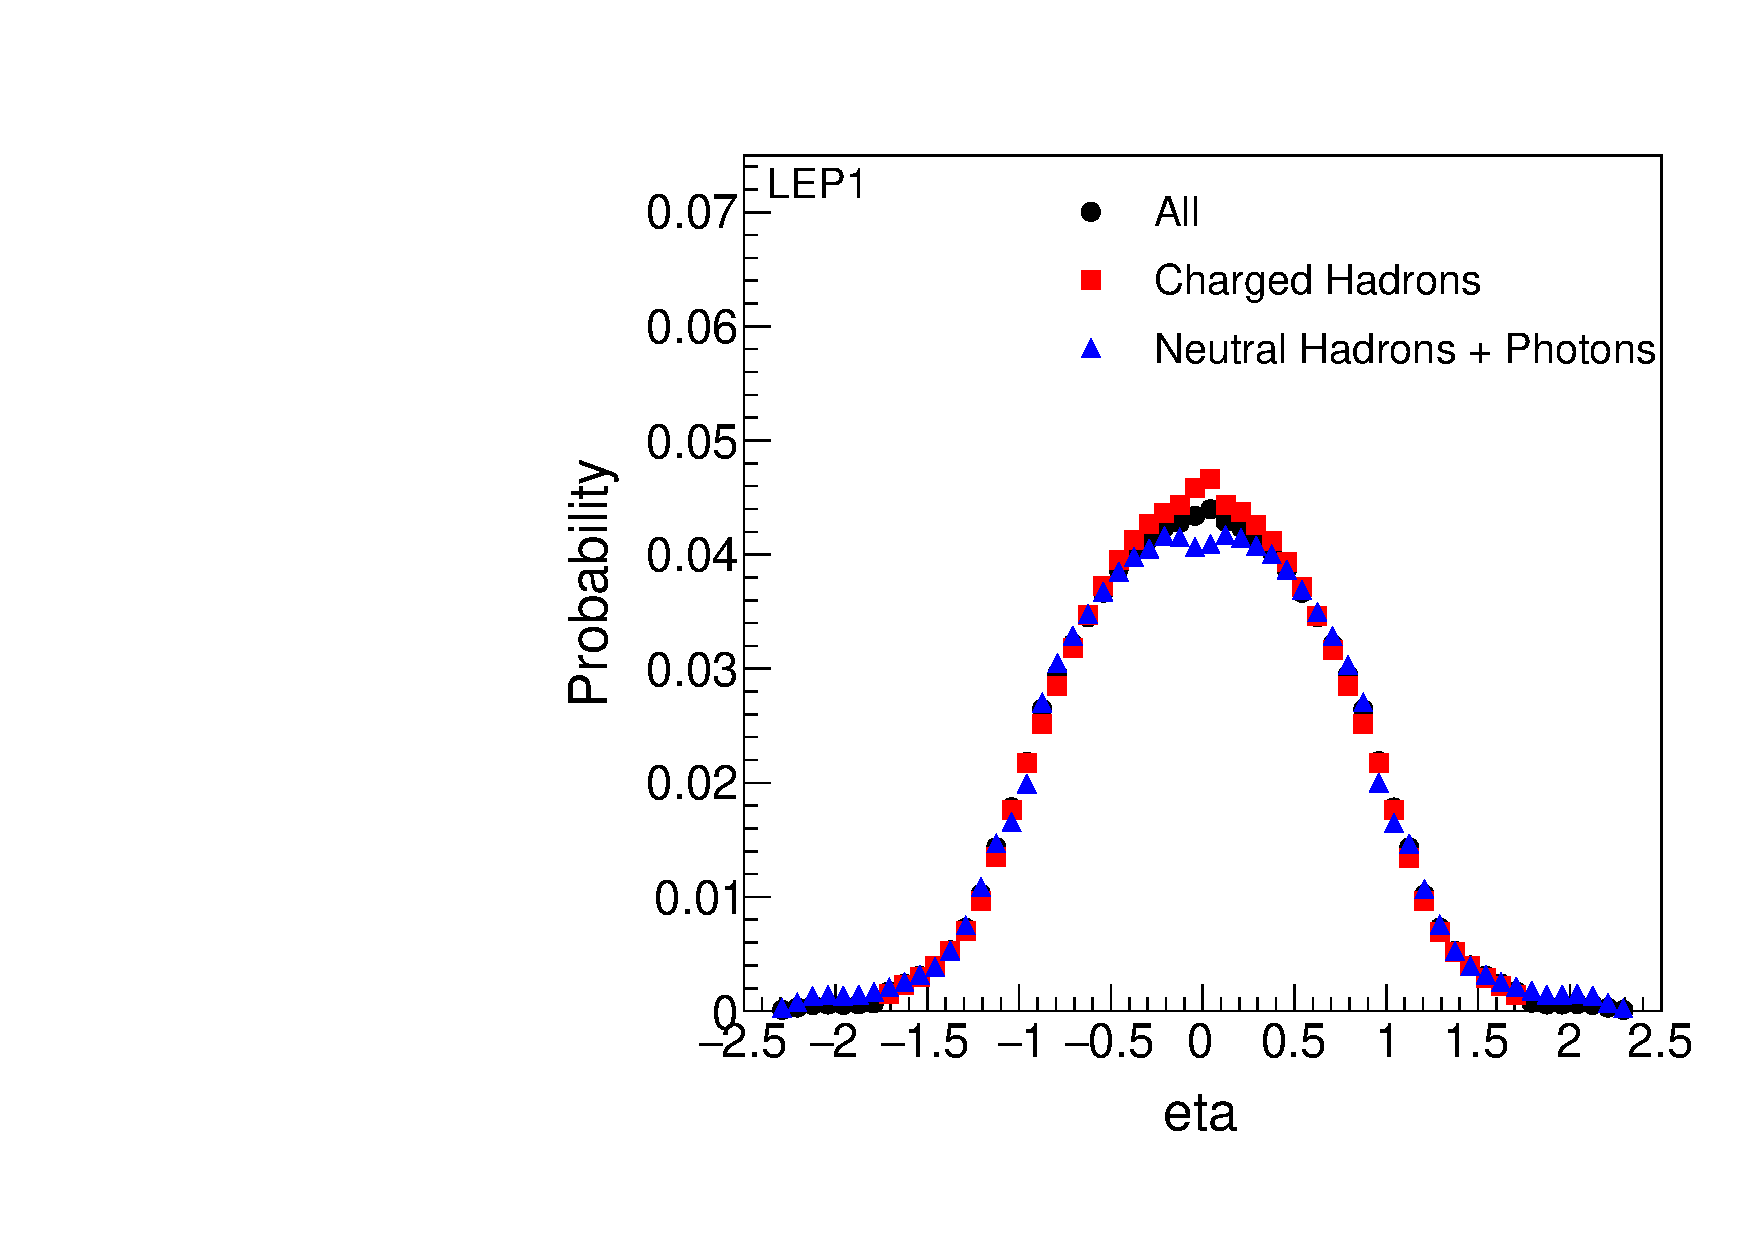
\includegraphics[width=.45\textwidth]{images/DataQualityCheck/LEP1_eta.pdf}
\caption{LEP1 Eta Spectra}
\label{fig:figure1} 
\end{center}
\end{figure}

\begin{figure}[!htb]
\begin{center}
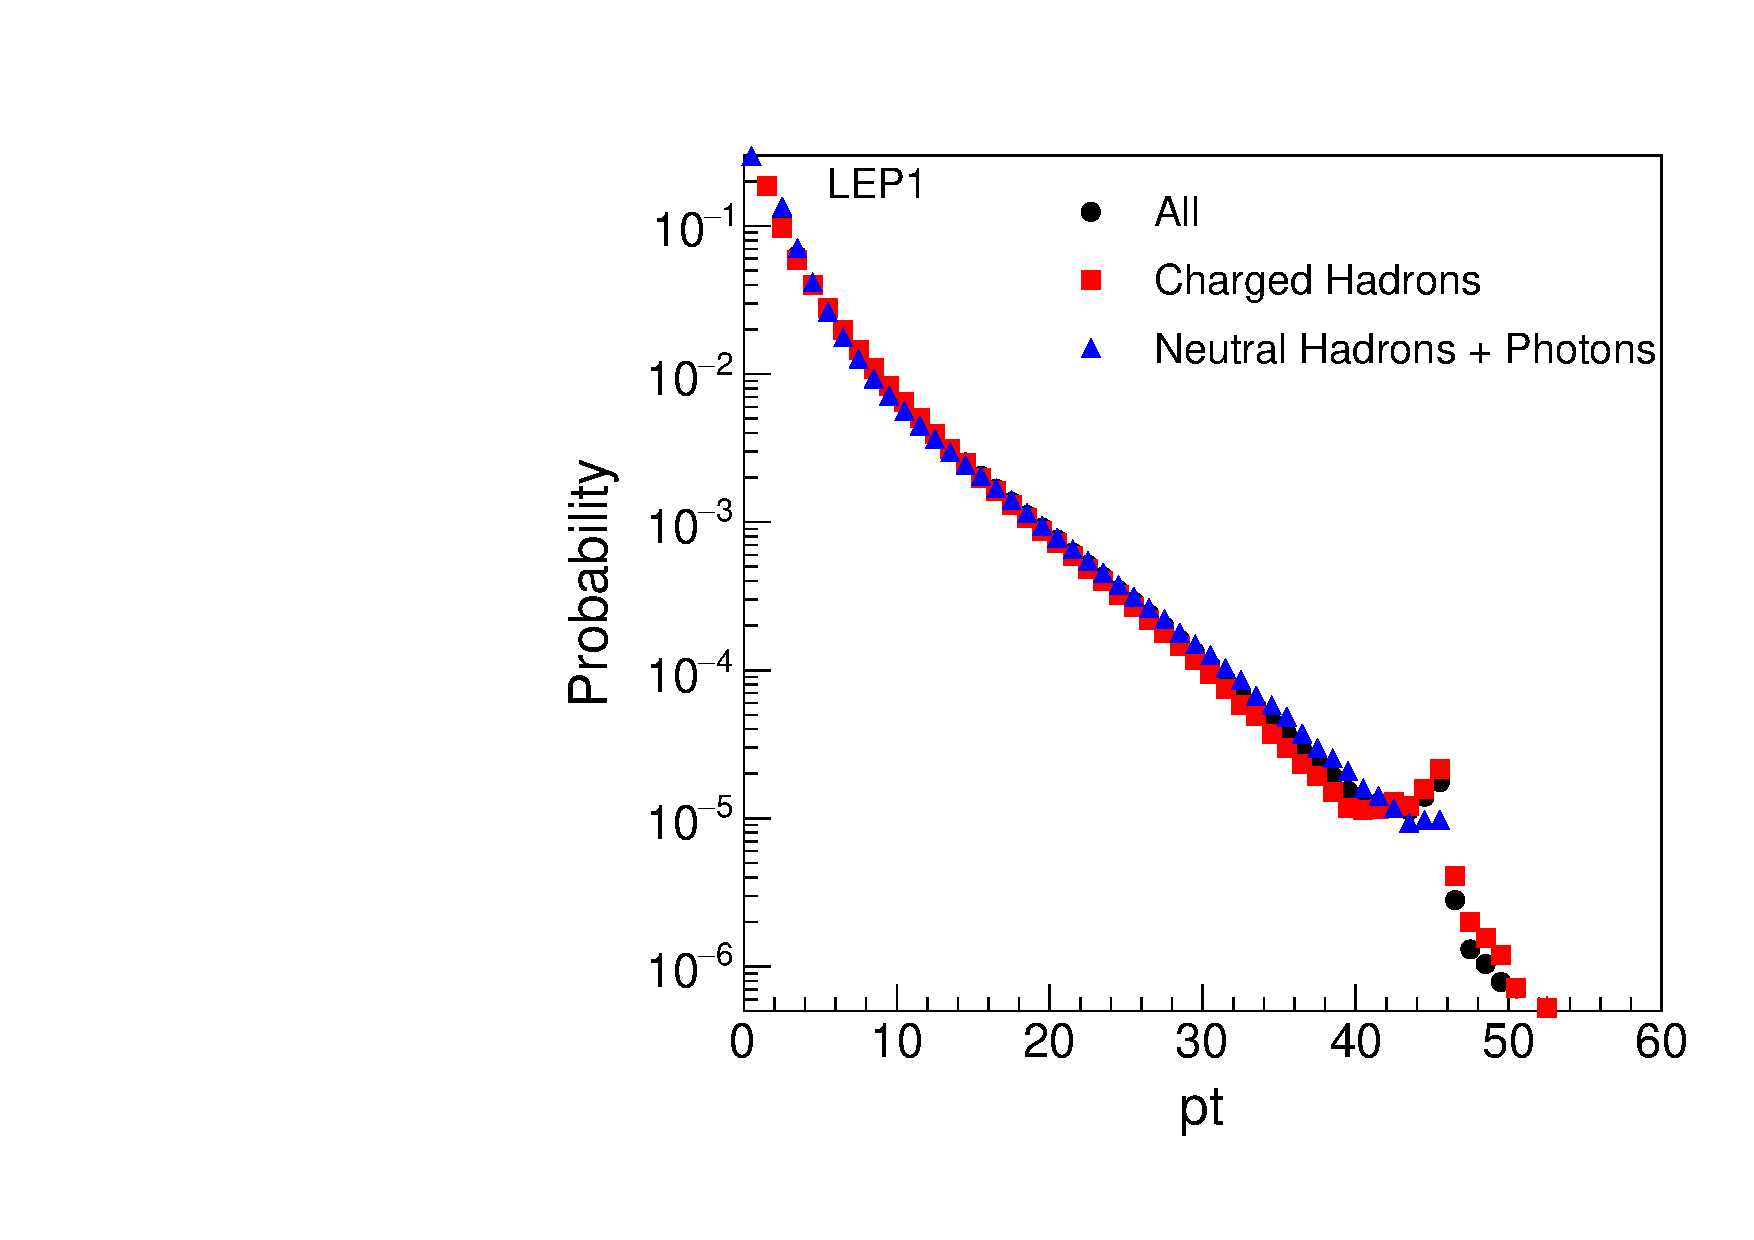
\includegraphics[width=.45\textwidth]{images/DataQualityCheck/LEP1_pt.pdf}
\caption{LEP1 PT spectra}
\label{fig:figure2} 
\end{center}
\end{figure}

\begin{figure}[!htb]
\begin{center}
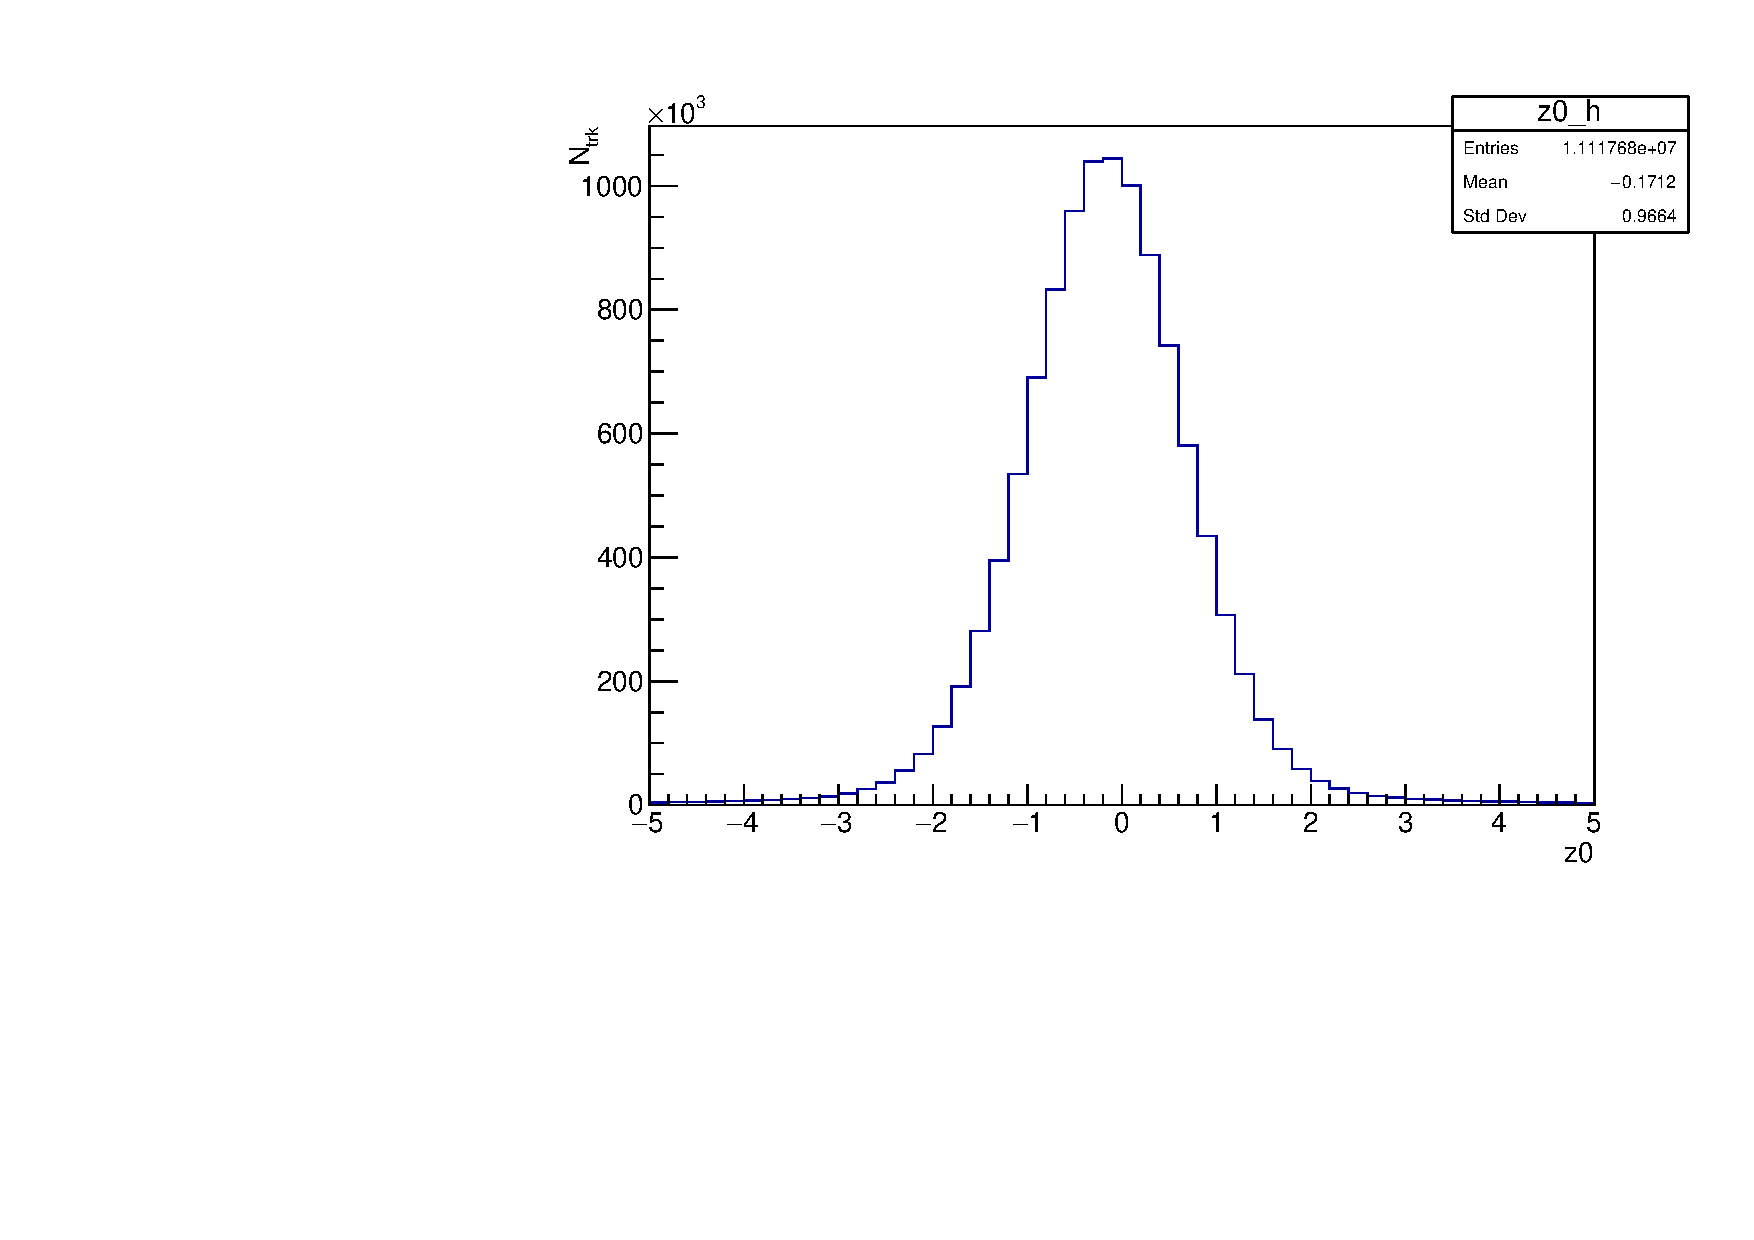
\includegraphics[width=.45\textwidth]{images/DataQualityCheck/z0.pdf}
\caption{LEP1 z distance-of-closest-approach distribution of charged tracks.}
\label{fig:z0} 
\end{center}
\end{figure}

\begin{figure}[!htb]
\begin{center}
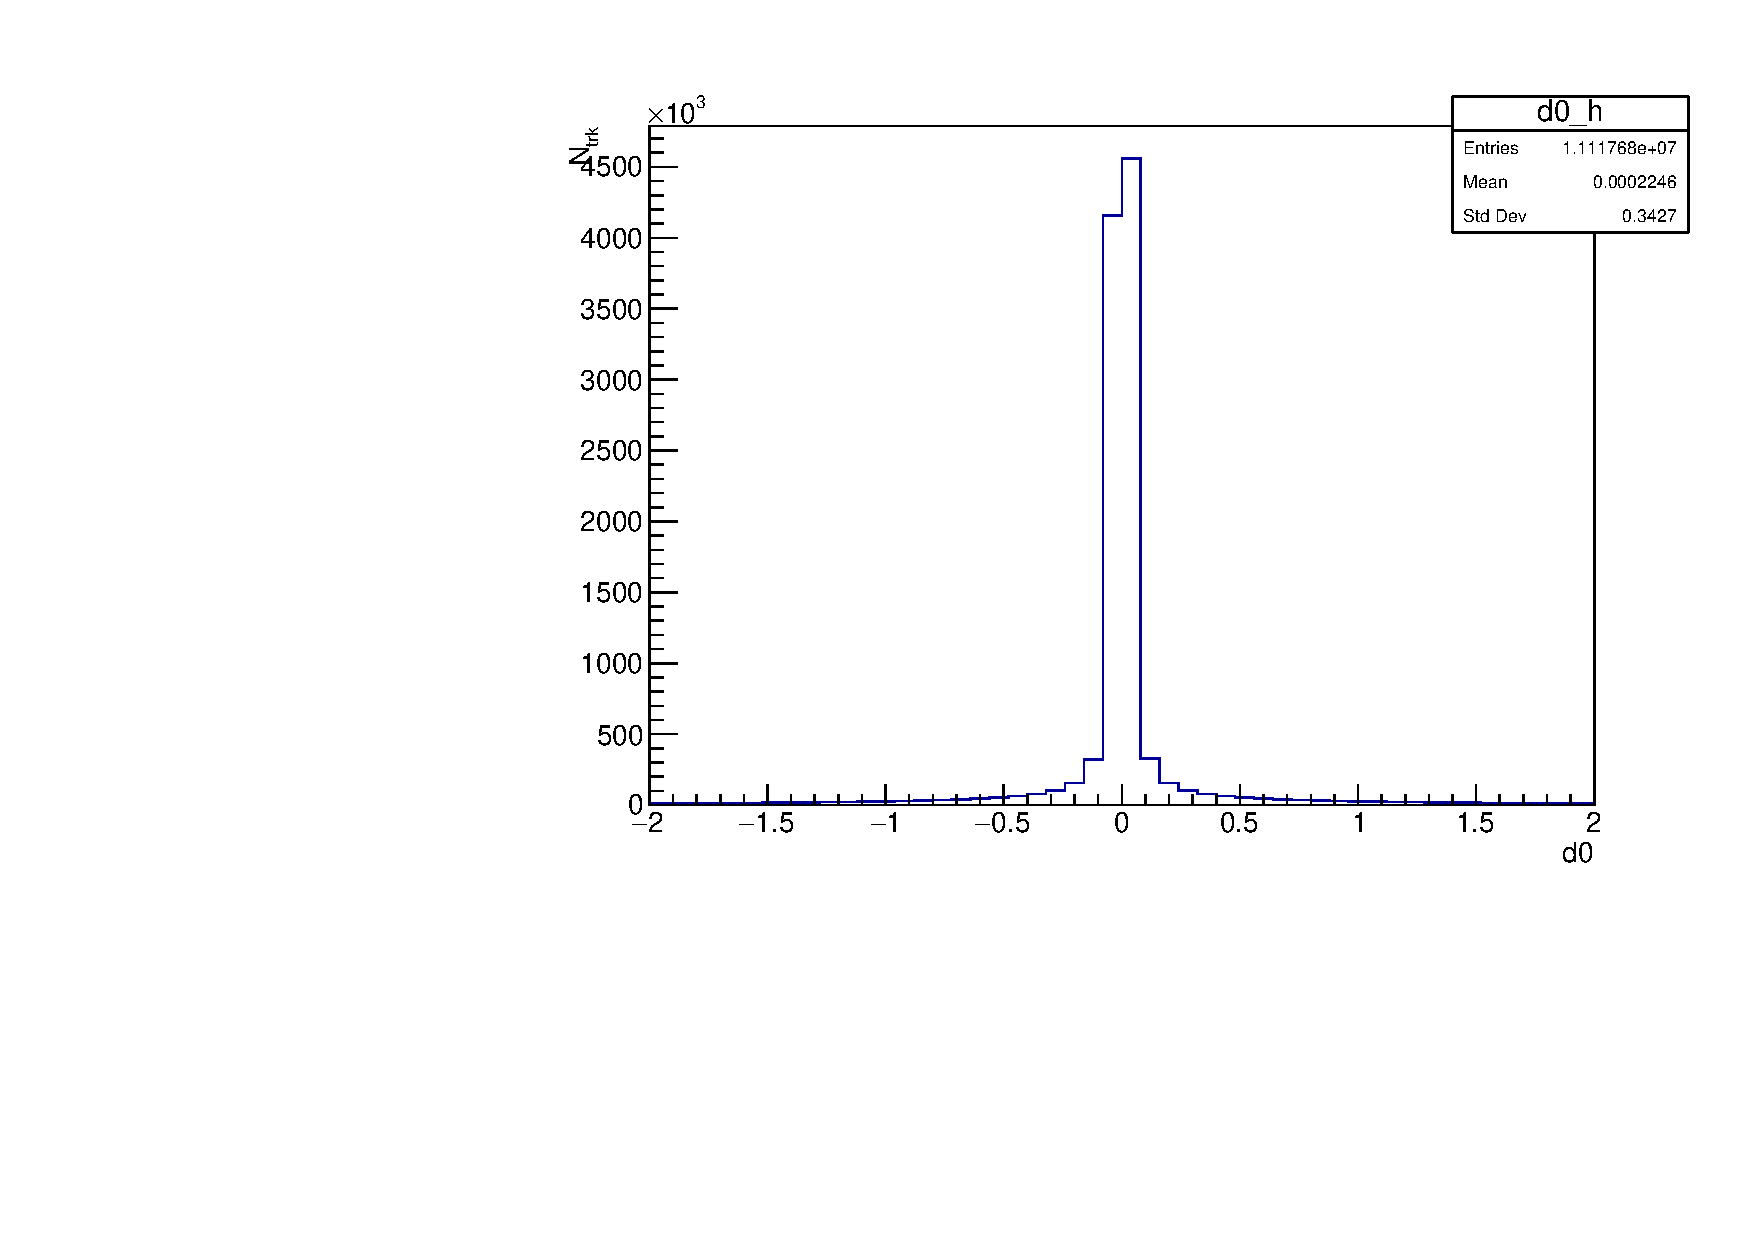
\includegraphics[width=.45\textwidth]{images/DataQualityCheck/d0.pdf}
\caption{LEP1 d0 distribution of charged tracks.}
\label{fig:d0} 
\end{center}
\end{figure}
\begin{figure}[!htb]

\begin{center}
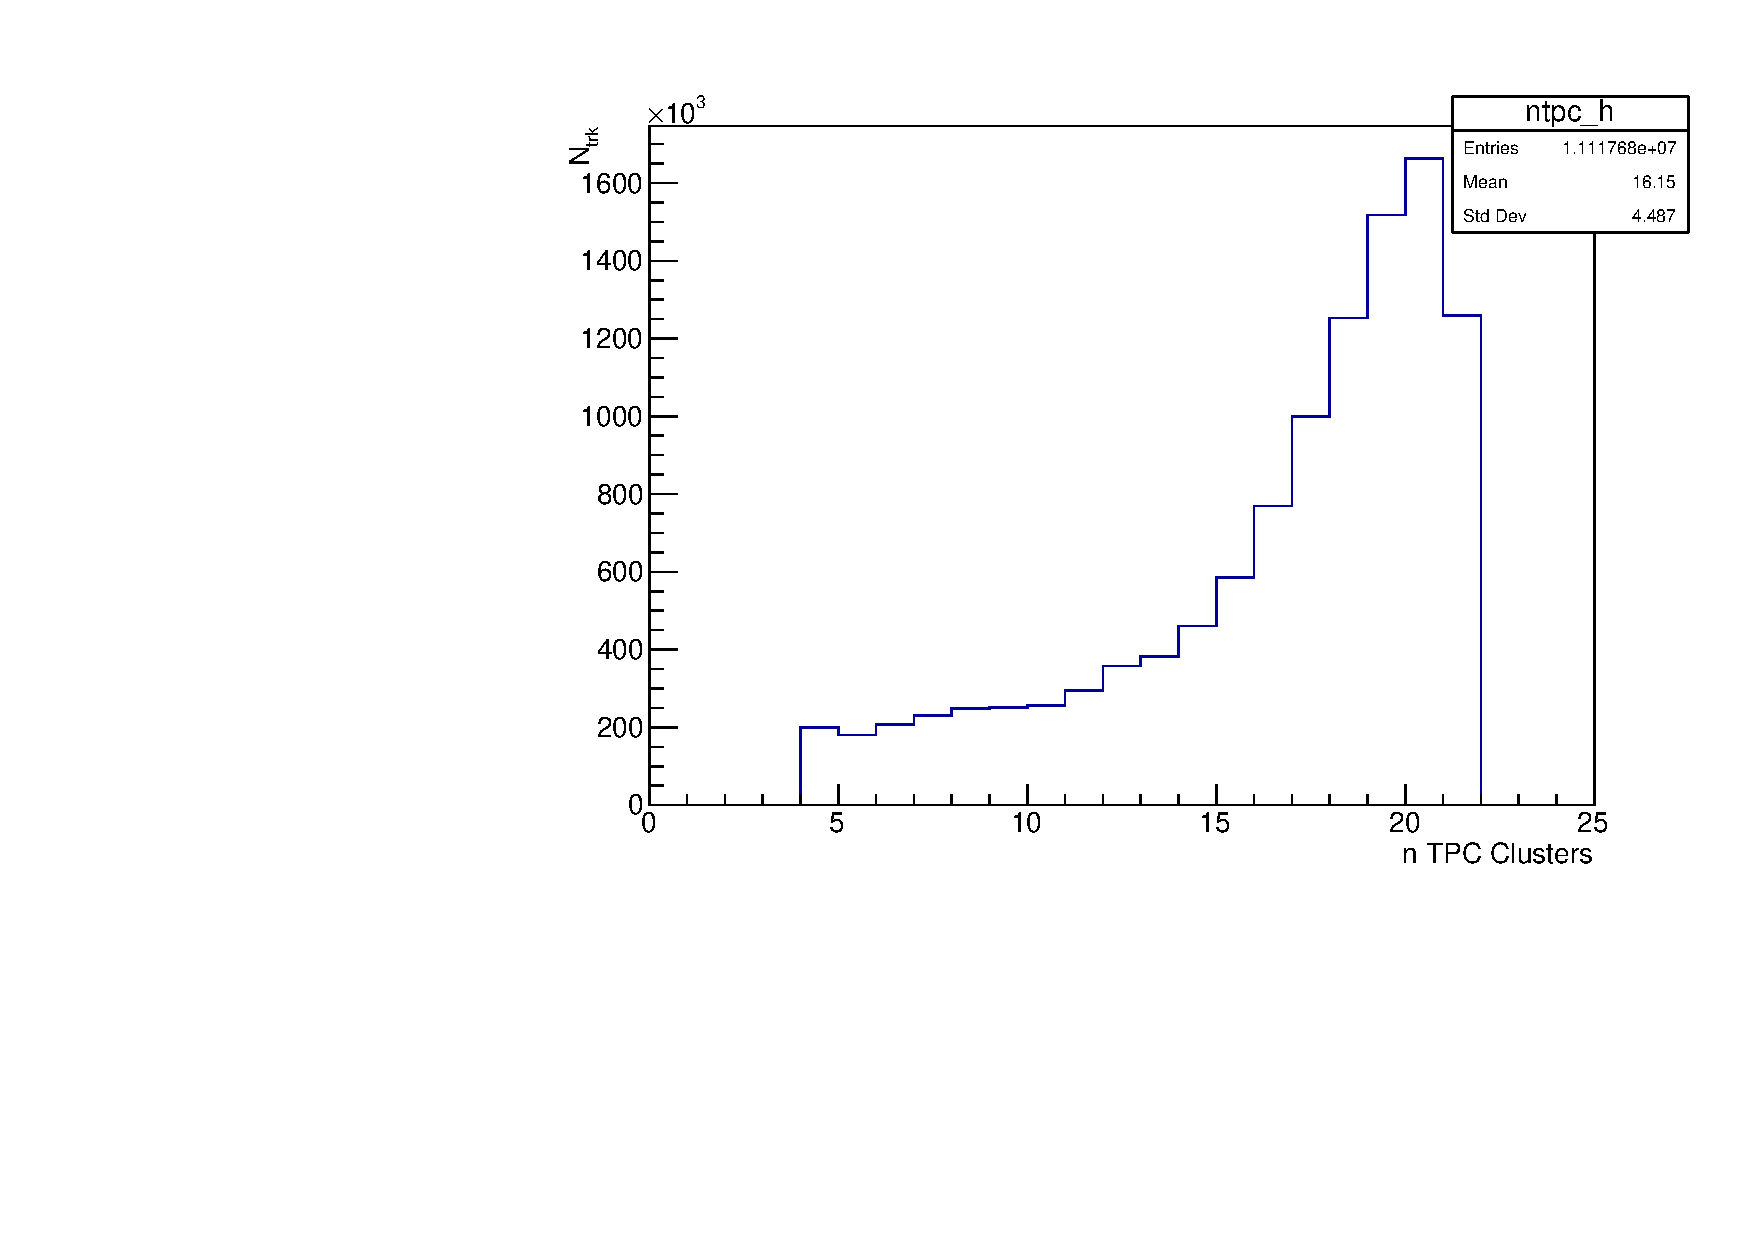
\includegraphics[width=.45\textwidth]{images/DataQualityCheck/ntpc.pdf}
\caption{LEP1 distribution of number of TPC clusters on charged tracks.}
\label{fig:ntpc} 
\end{center}
\end{figure}

%%%%%%%%%%%%%%%%%%%%%%%%%%%%%%%%%%%% LEP 2 %%%%%%%%%%%%%%%%%%%%%%%%%%%%%%%%
\begin{figure}[!htb]
\begin{center}
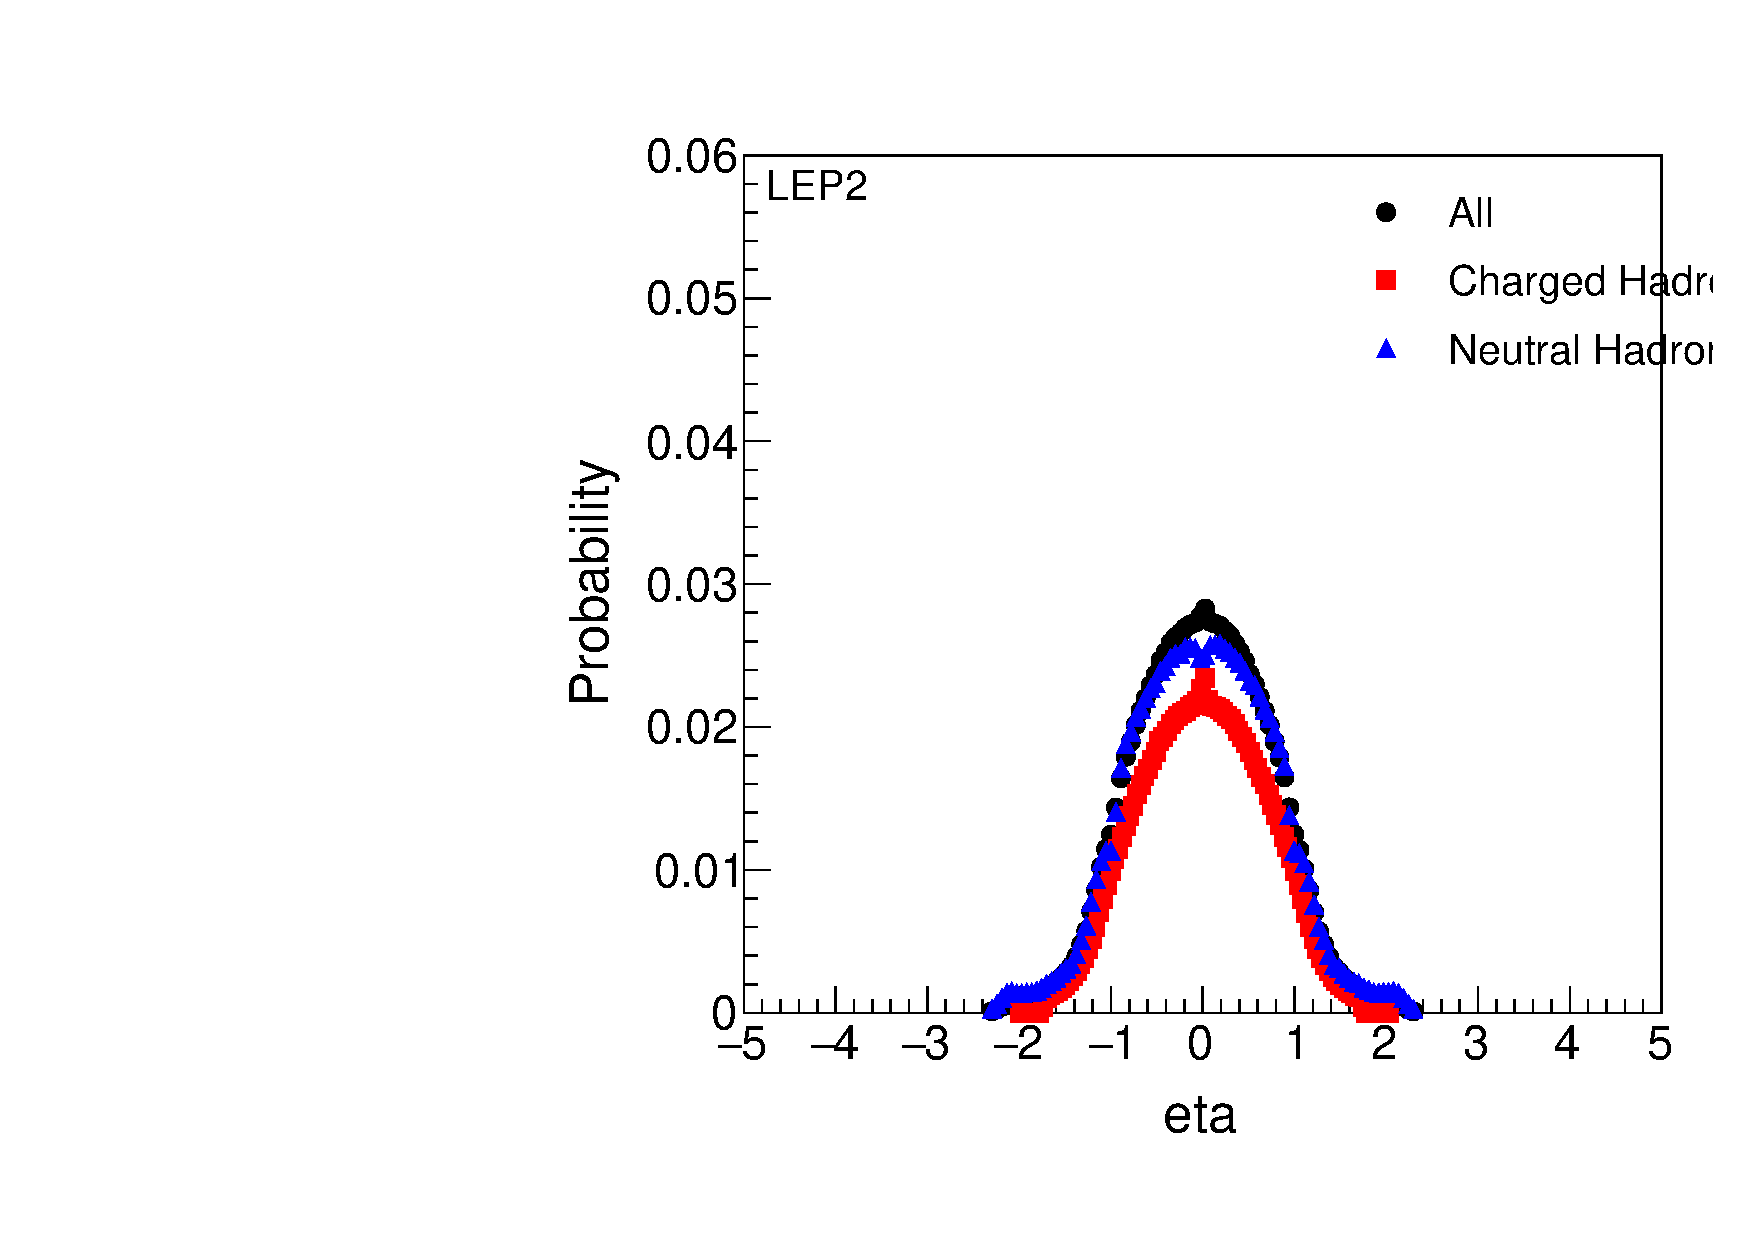
\includegraphics[width=.45\textwidth]{images/DataQualityCheck/LEP2_eta.pdf}
\caption{LEP2 Eta Spectra}
\label{fig:figure4} 
\end{center}
\end{figure}

\begin{figure}[!htb]
\begin{center}
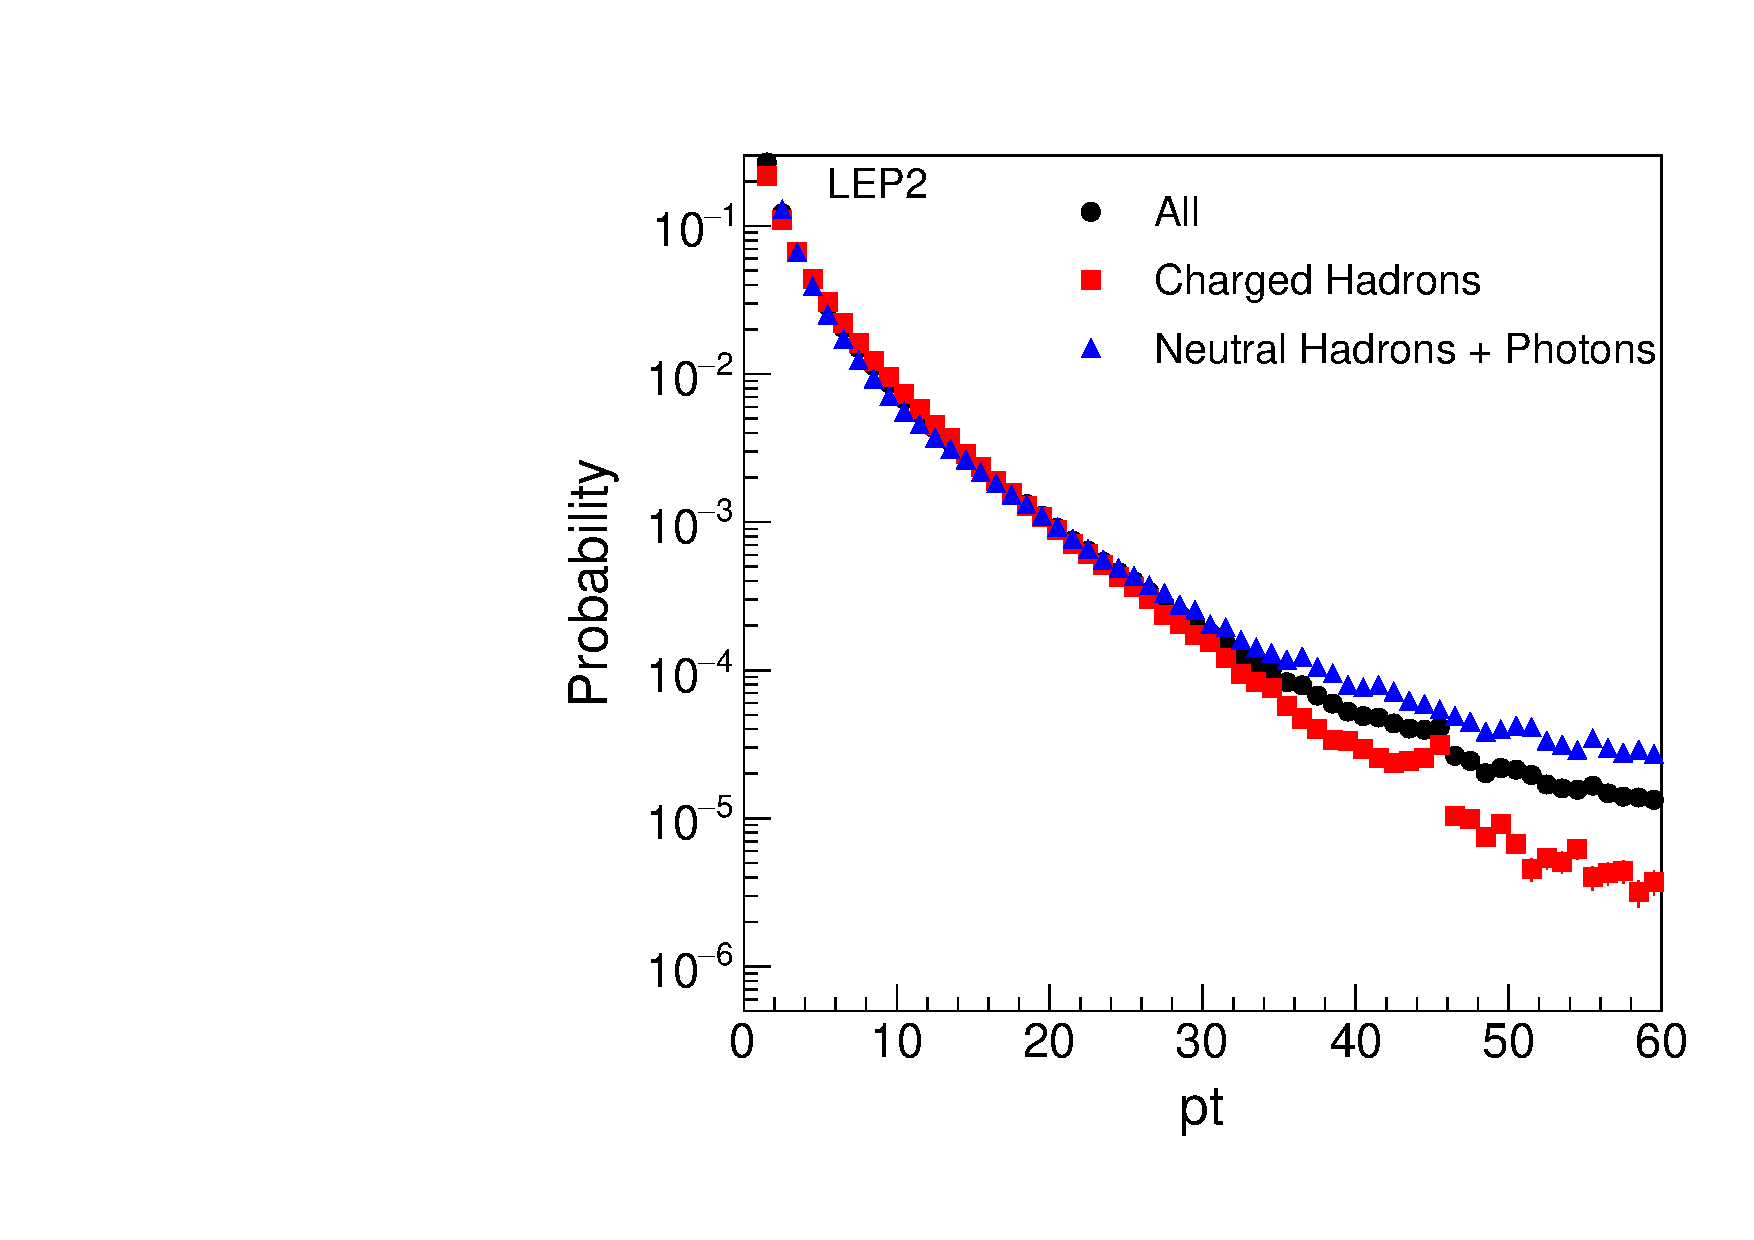
\includegraphics[width=.45\textwidth]{images/DataQualityCheck/LEP2_pt.pdf}
\caption{LEP2 PT spectra}
\label{fig:figure5} 
\end{center}
\end{figure}

\begin{figure}[!htb]
\begin{center}
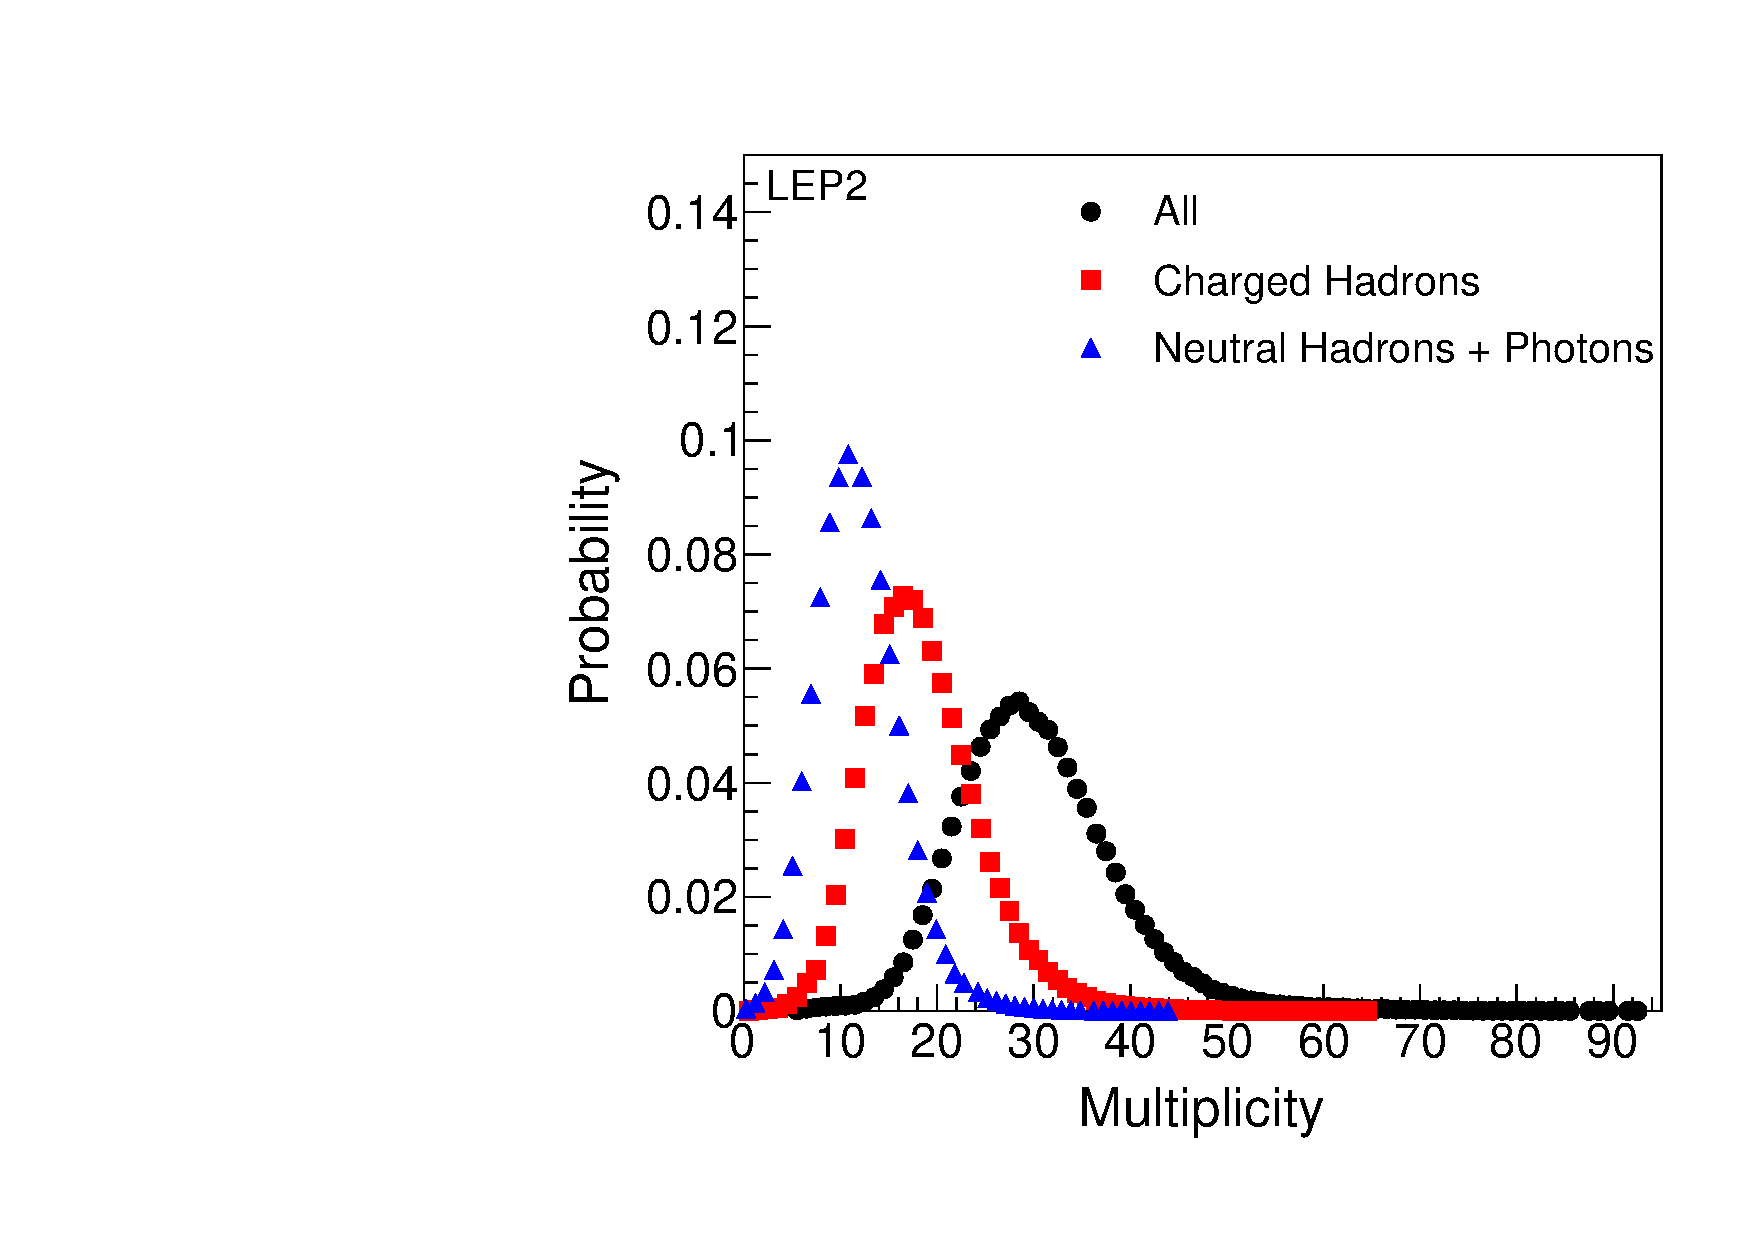
\includegraphics[width=.45\textwidth]{images/DataQualityCheck/LEP2_mult.pdf}
\caption{LEP2 Multiplicity Distribution}
\label{fig:figure6} 
\end{center}
\end{figure}

%%%%%%%%%%%%%%%%%%%%%%%%%%%%%%%%%%%% PYTHIA8 %%%%%%%%%%%%%%%%%%%%%%%%%%%%%%%%
\begin{figure}[!htb]
\begin{center}
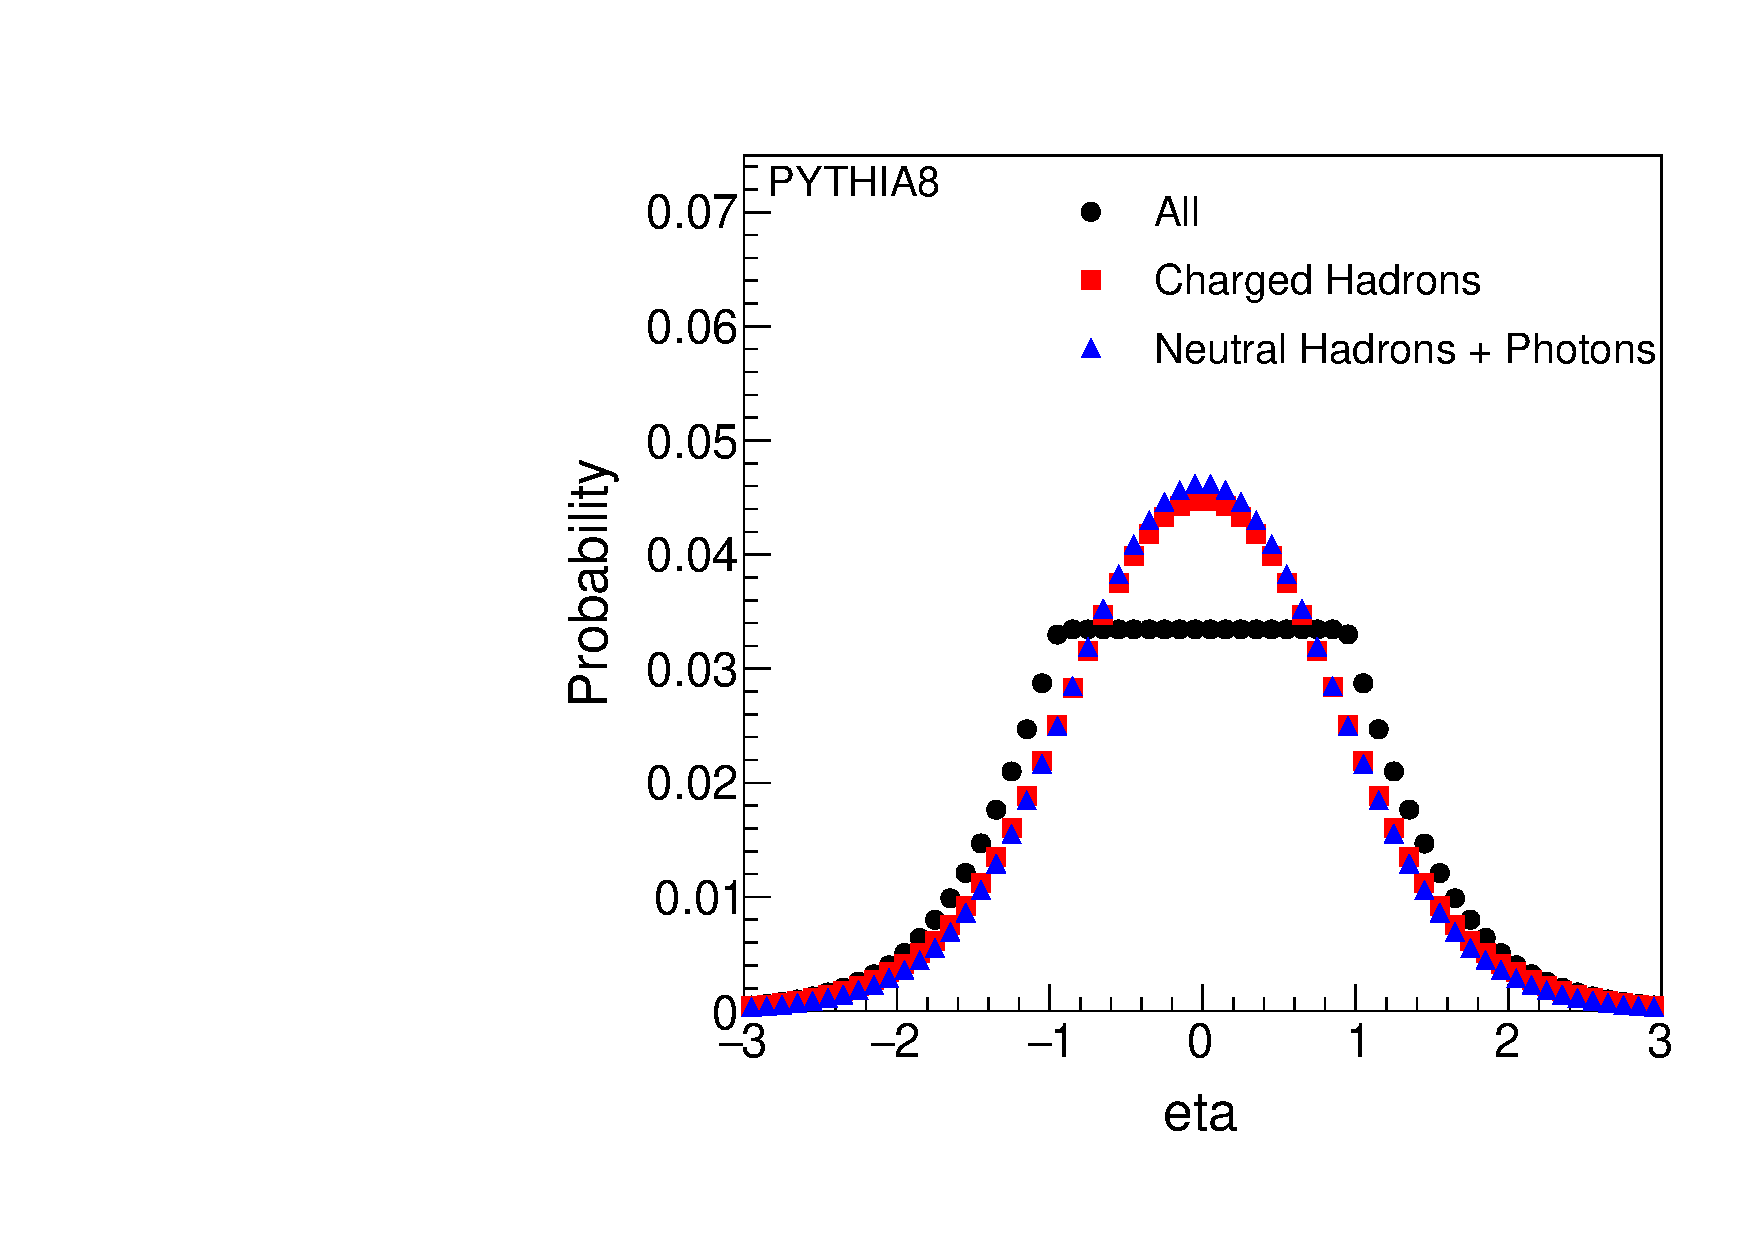
\includegraphics[width=.45\textwidth]{images/DataQualityCheck/PYTHIA8_eta.pdf}
\caption{PYTHIA8 Eta Spectra}
\label{fig:figure7} 
\end{center}
\end{figure}

\begin{figure}[!htb]
\begin{center}
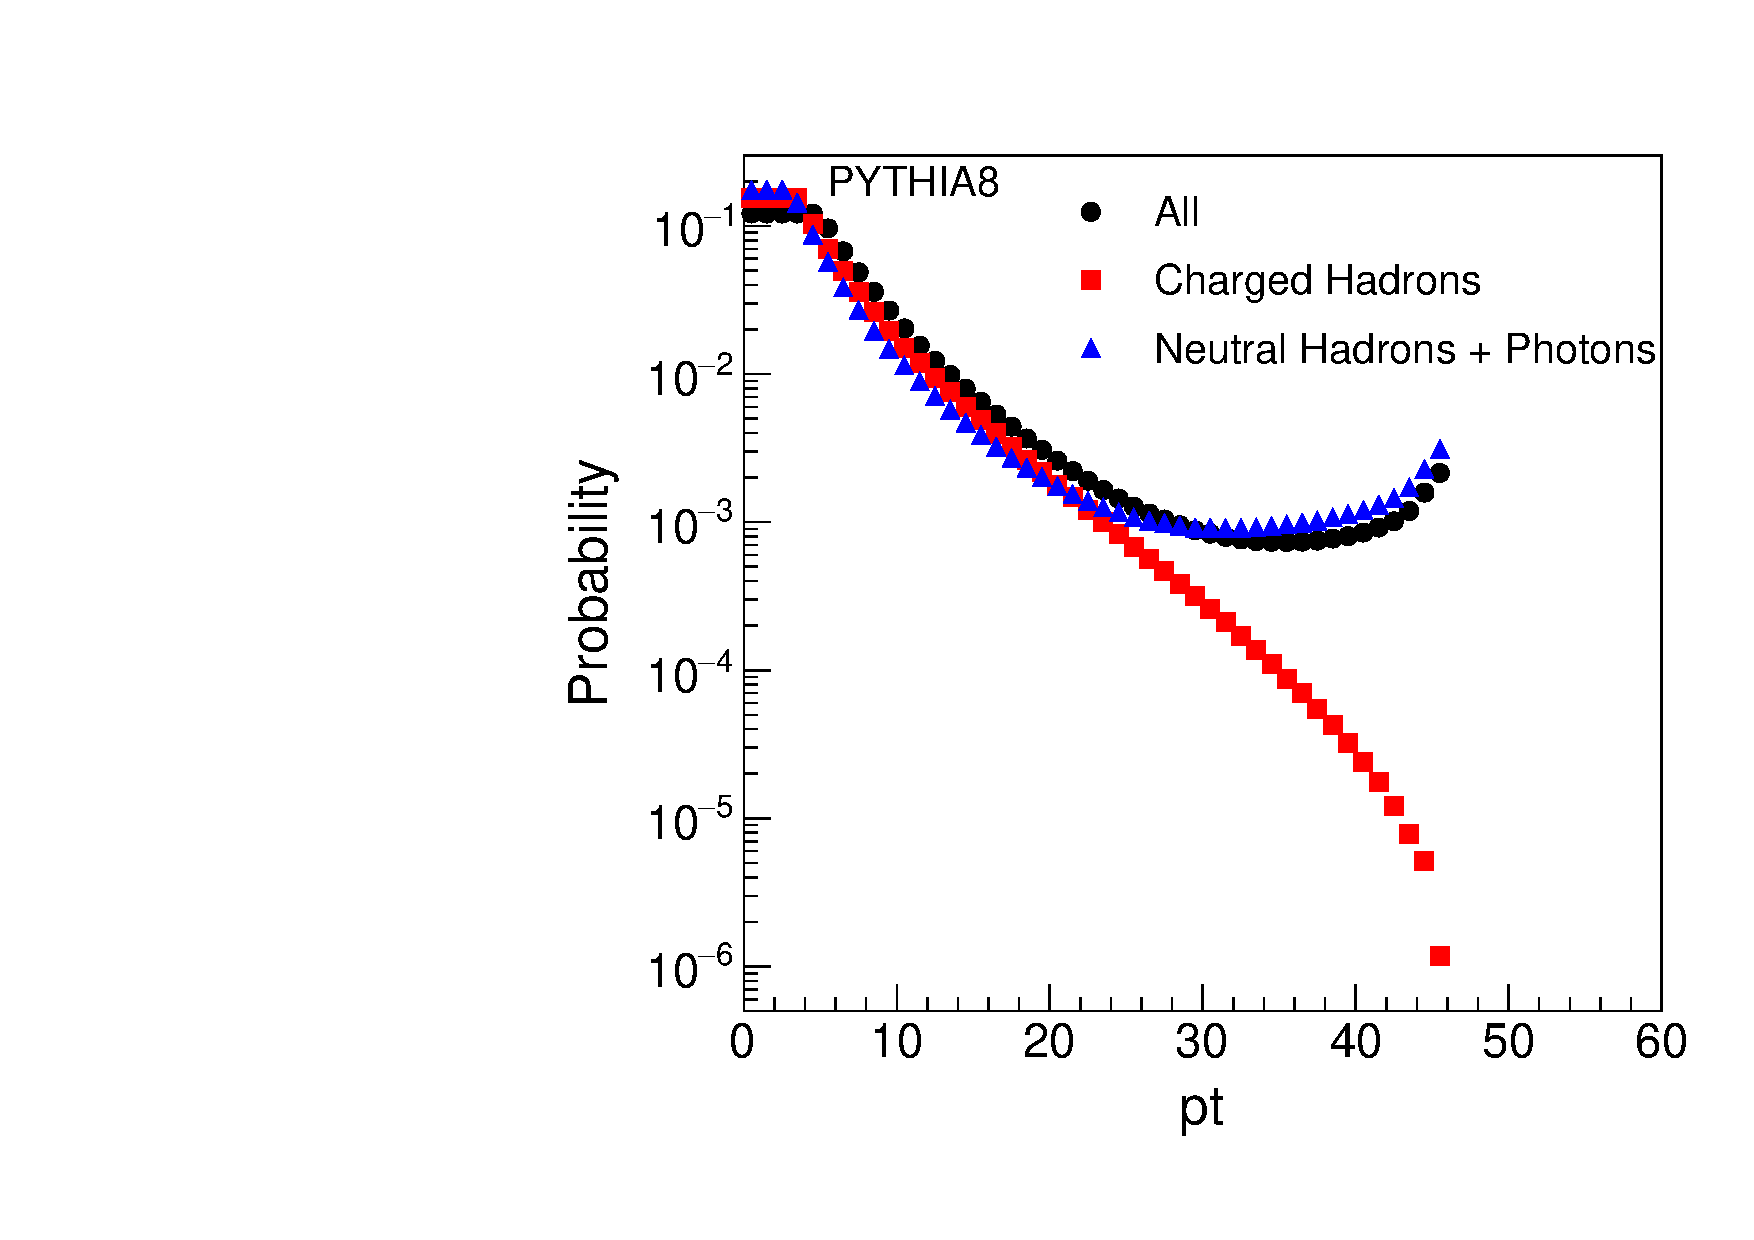
\includegraphics[width=.45\textwidth]{images/DataQualityCheck/PYTHIA8_pt.pdf}
\caption{PYTHIA8 PT spectra}
\label{fig:figure8} 
\end{center}
\end{figure}

\begin{figure}[!htb]
\begin{center}
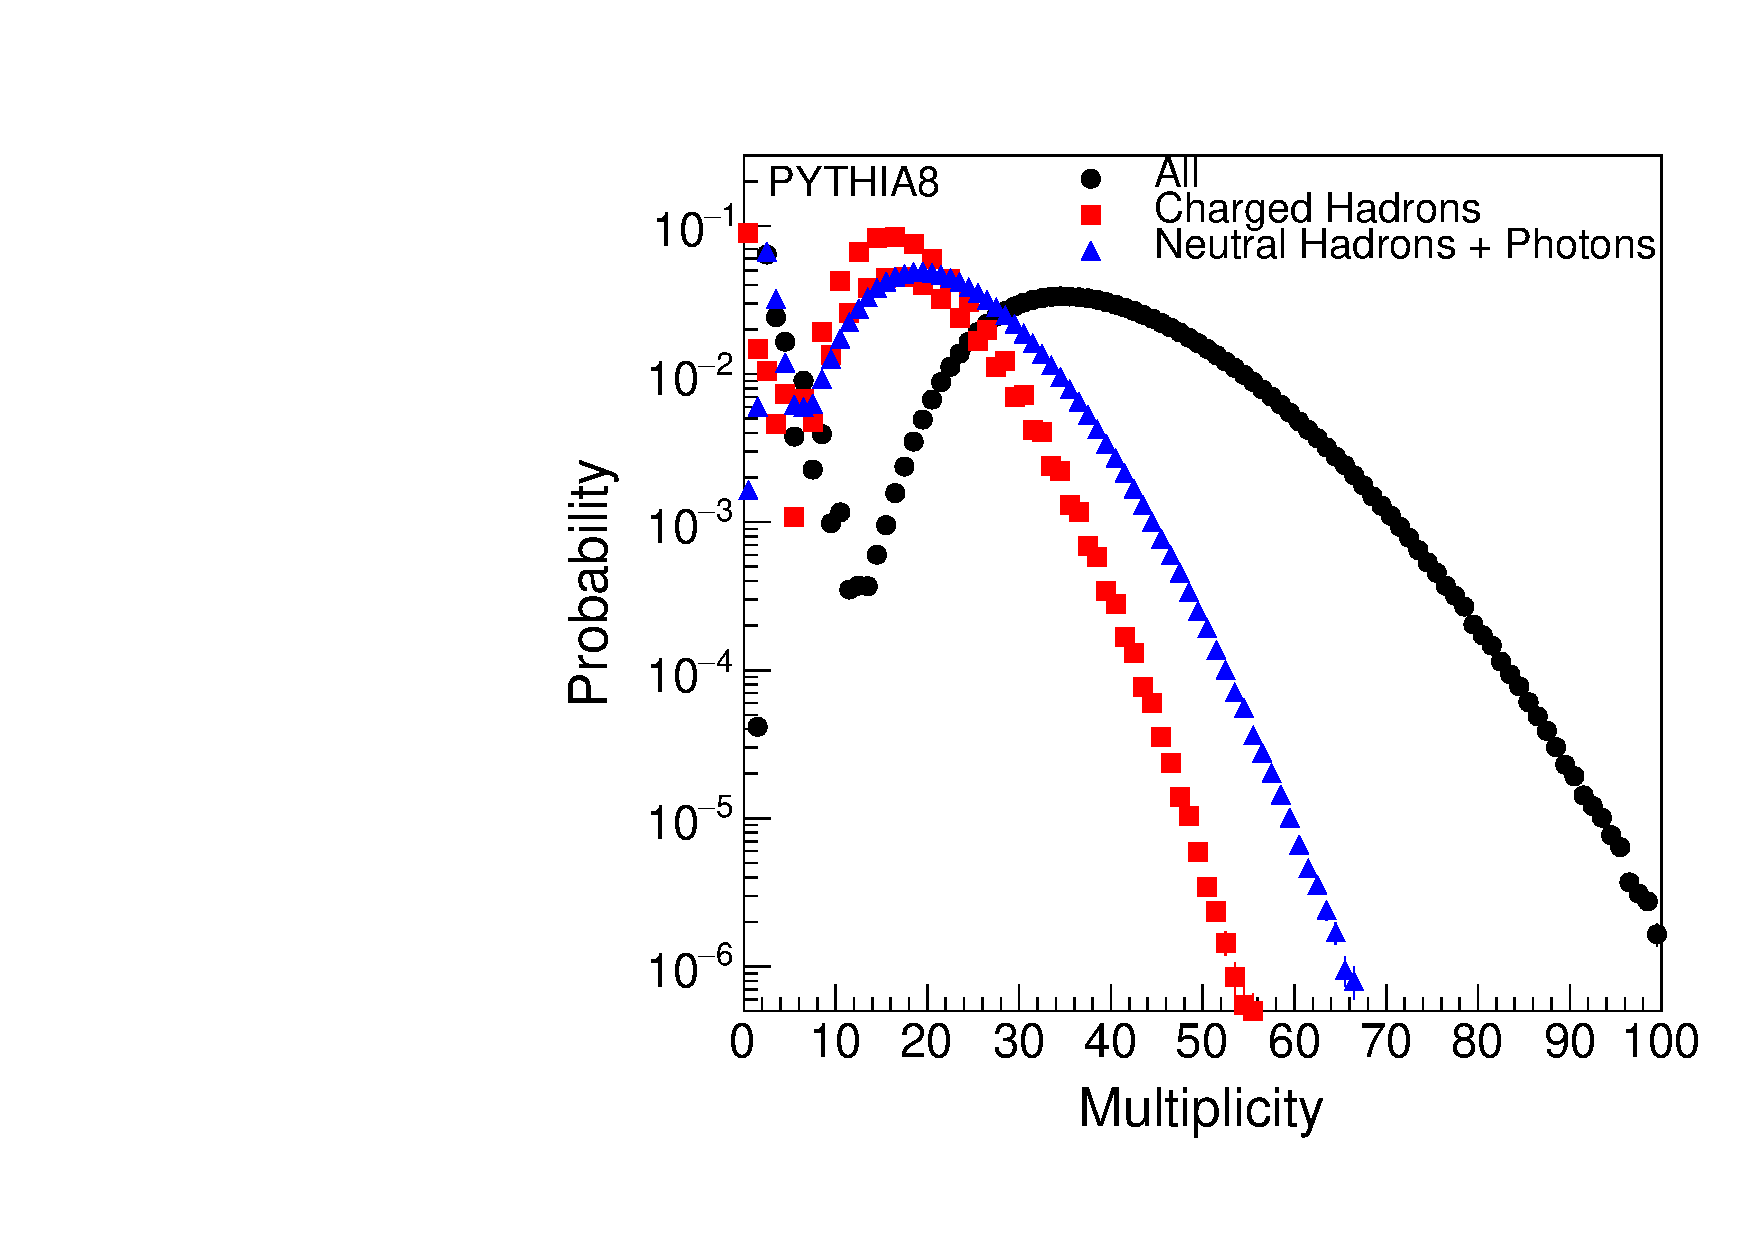
\includegraphics[width=.45\textwidth]{images/DataQualityCheck/PYTHIA8_mult.pdf}
\caption{PYTHIA8 Multiplicity Distribution}
\label{fig:figure9} 
\end{center}
\end{figure}

%%%%%%%%%%%%%%%%%%%%%%%%%%%%% LEP 1 vs PYTHIA8 %%%%%%%%%%%%%%%%%%%%%%%%%%%%%
\begin{figure}[!htb]
\begin{center}
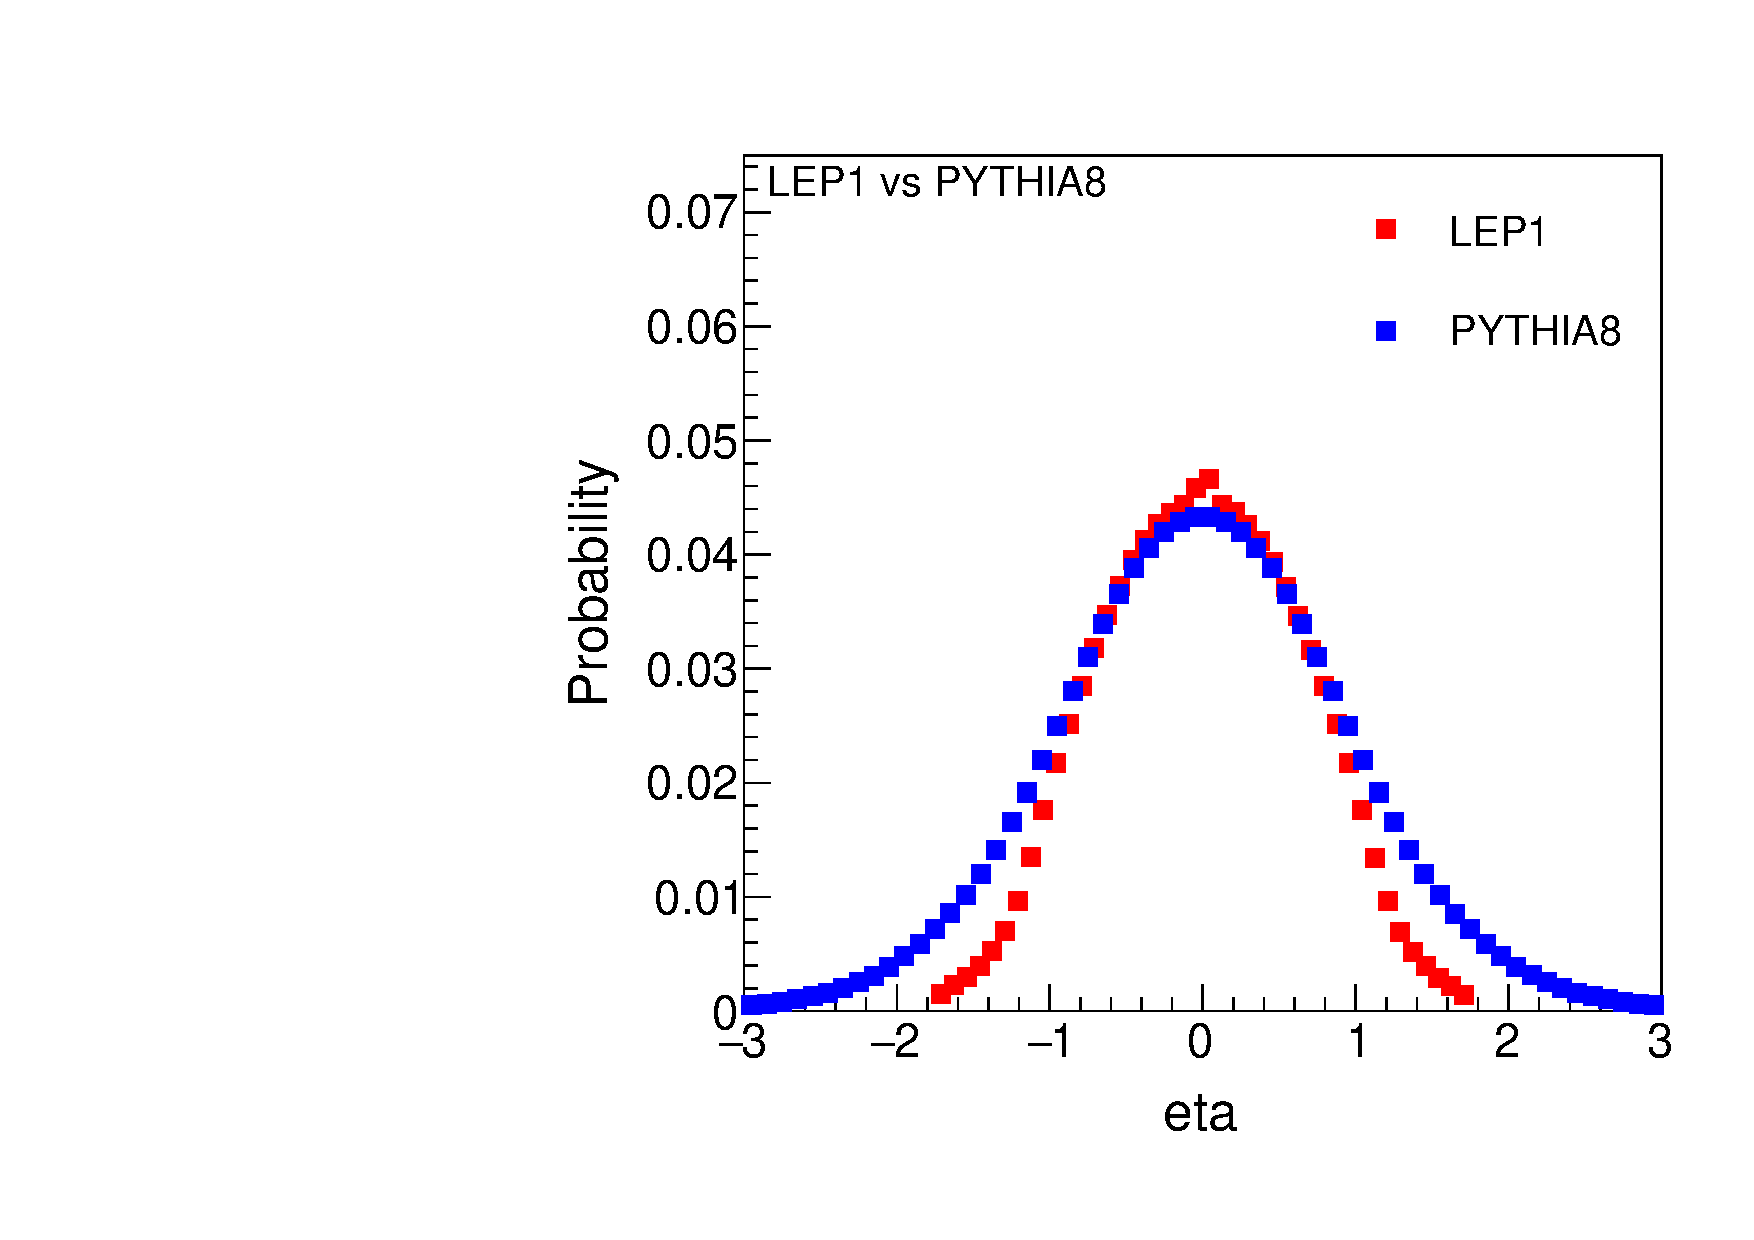
\includegraphics[width=.45\textwidth]{images/DataQualityCheck/eta_LEP1_PYTHIA8.pdf}
\caption{LEP1 vs PYTHIA8 Eta Spectra of charged hadrons}
\label{fig:figure10} 
\end{center}
\end{figure}

\begin{figure}[!htb]
\begin{center}
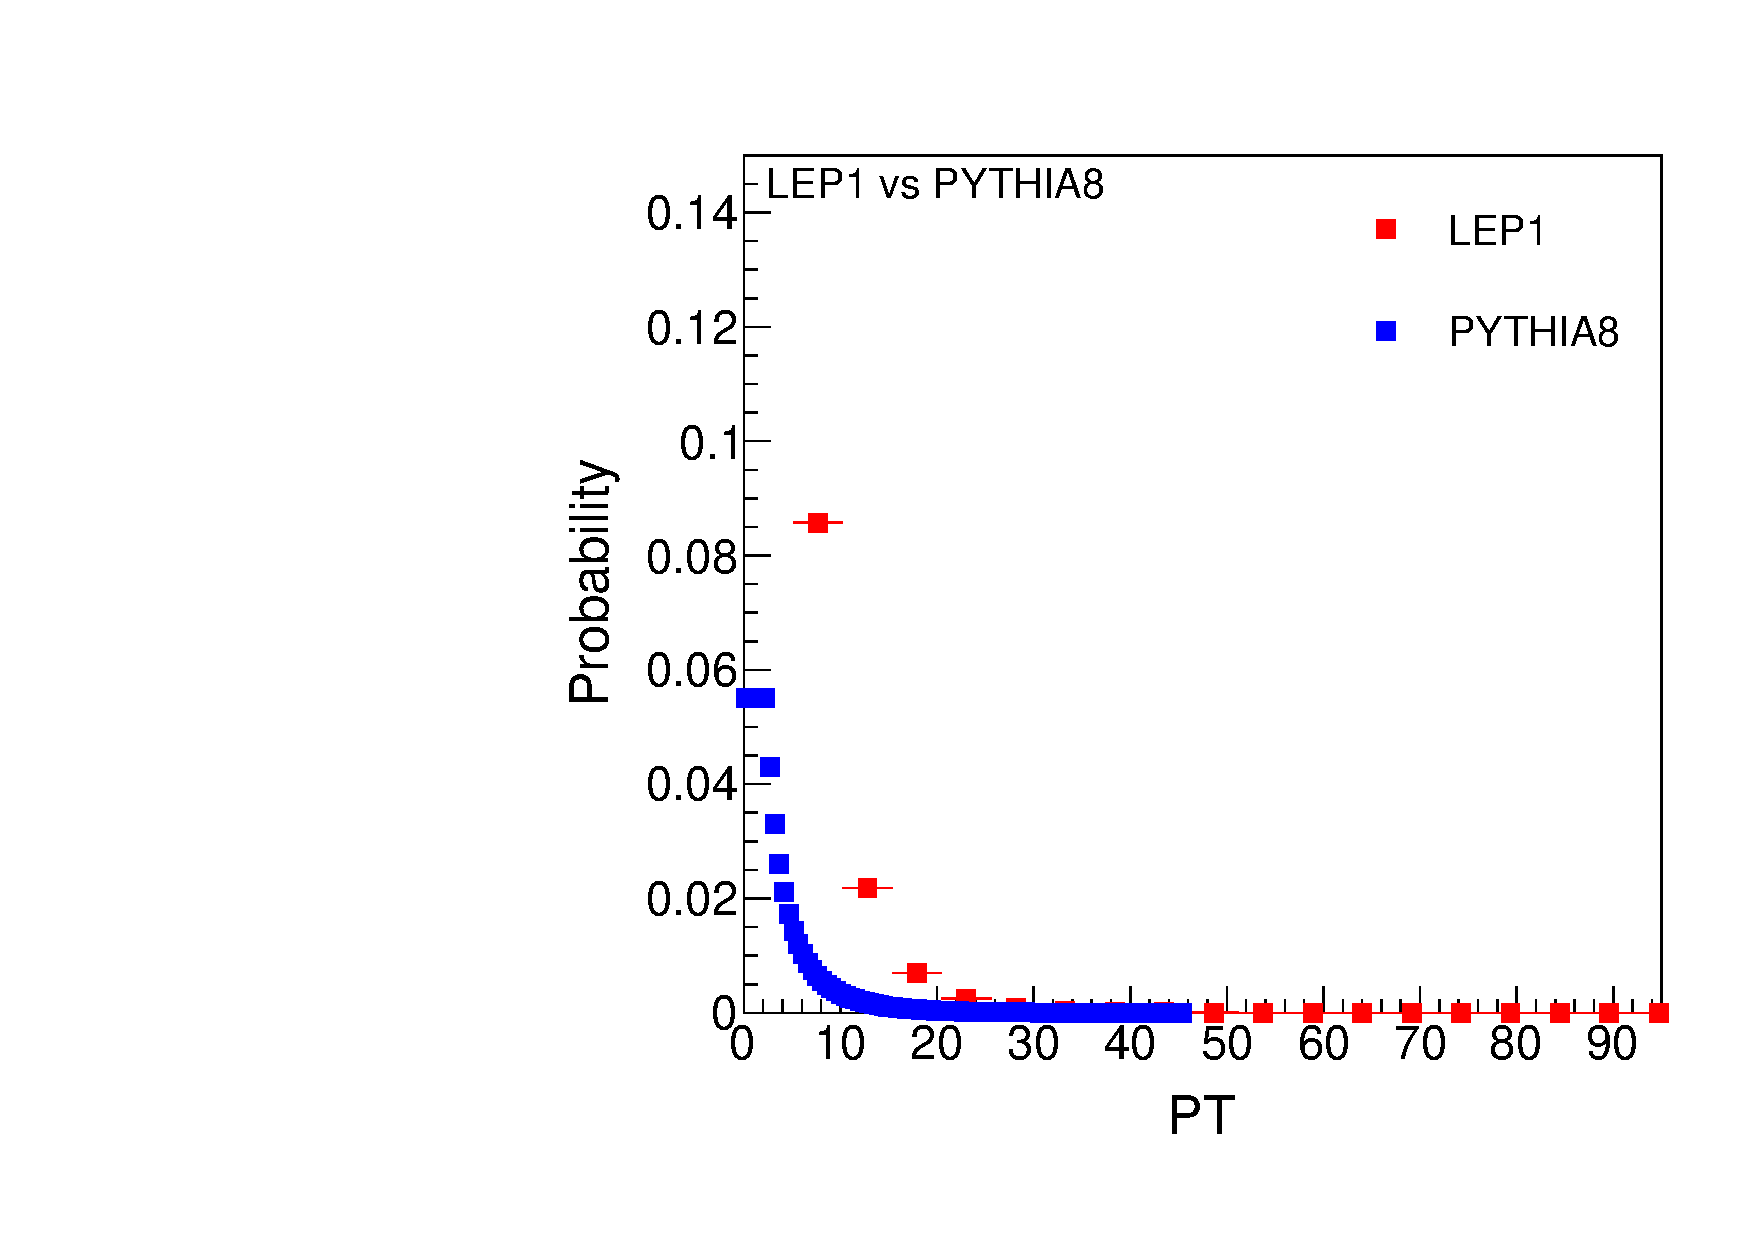
\includegraphics[width=.45\textwidth]{images/DataQualityCheck/pt_LEP1_PYTHIA8.pdf}
\caption{LEP1 vs PYTHIA8 PT spectra of charged hadrons}
\label{fig:figure11} 
\end{center}
\end{figure}

\begin{figure}[!htb]
\begin{center}
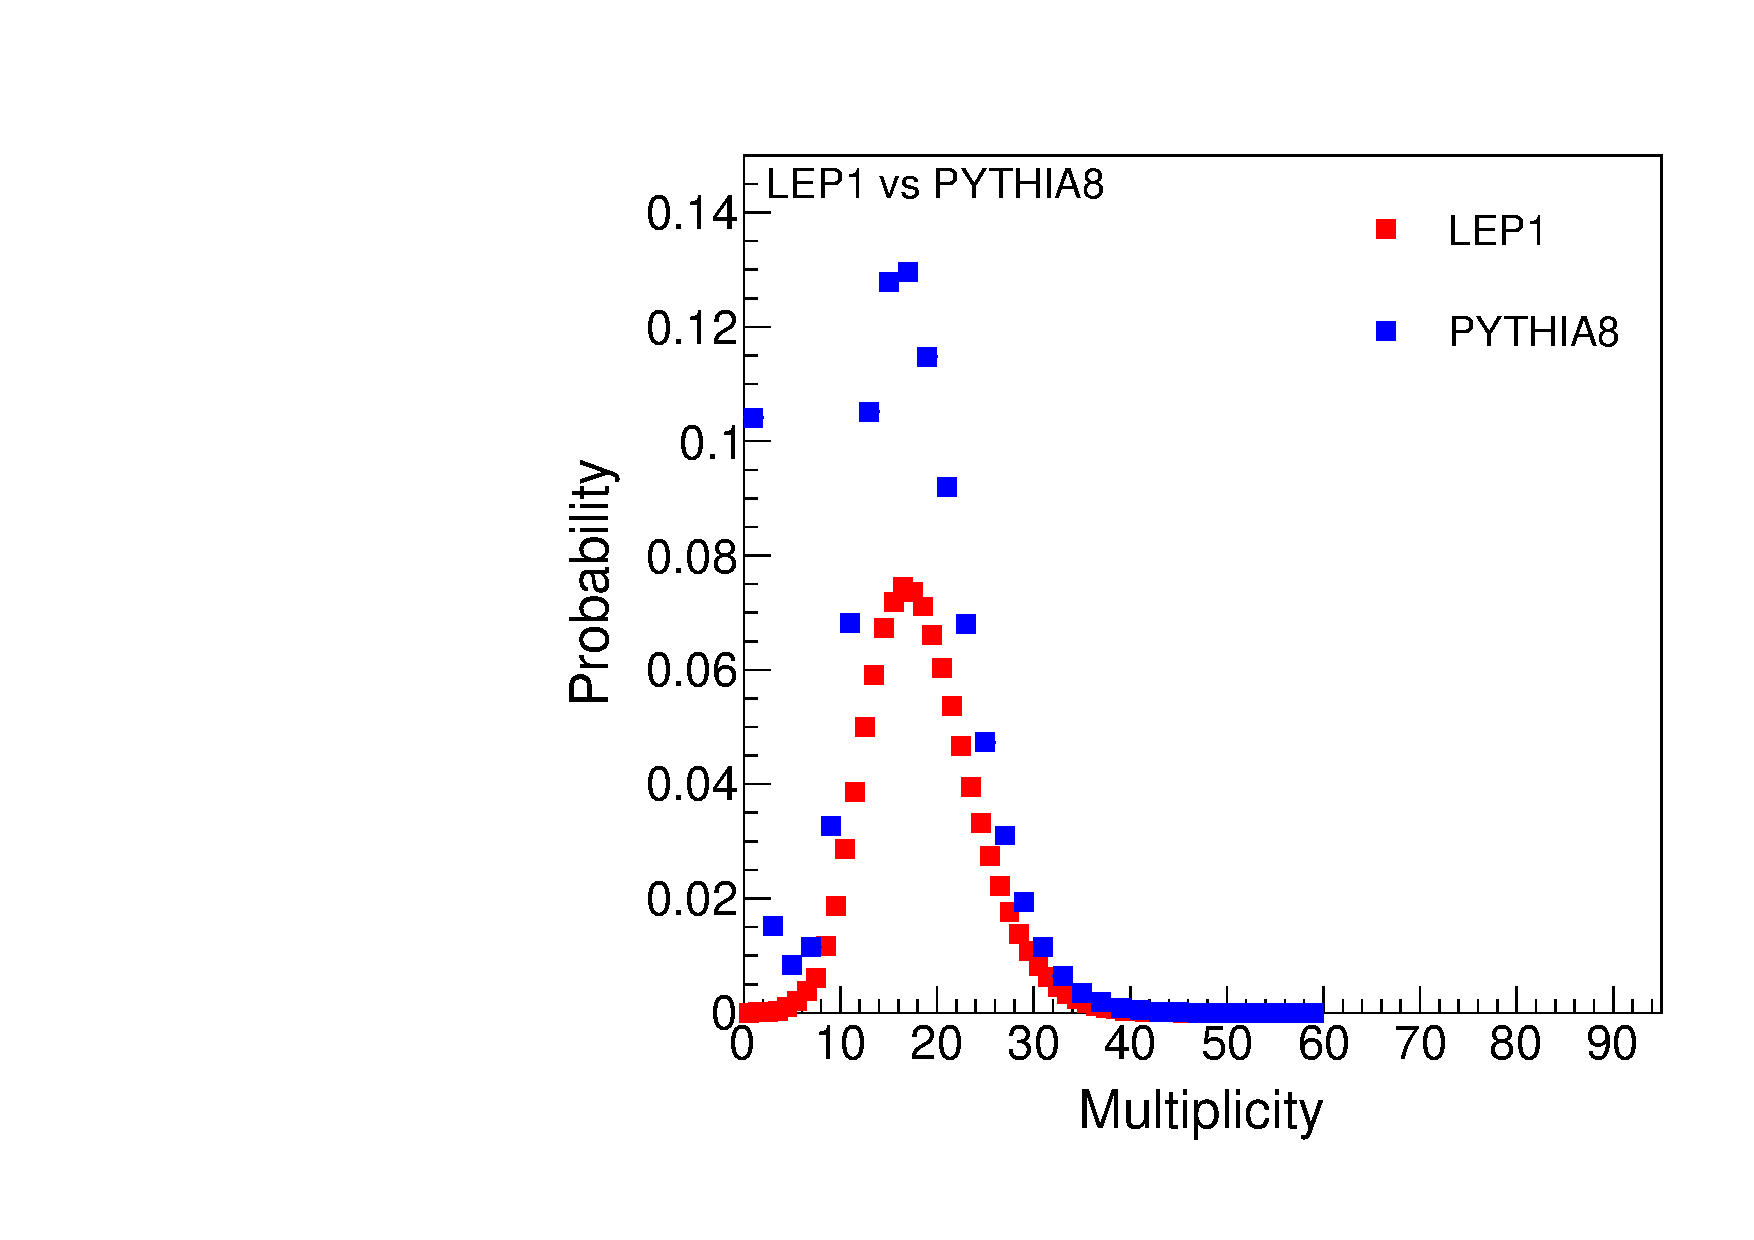
\includegraphics[width=.45\textwidth]{images/DataQualityCheck/mult_LEP1_PYTHIA8.pdf}
\caption{LEP1 vs PYTHIA8 Multiplicity Distribution of charged hadrons}
\label{fig:figure12} 
\end{center}
\end{figure}
